% ------------------------------------------------------------------------
% ------------------------------------------------------------------------
% abnTeX2: Modelo de Trabalho Academico (tese de doutorado, dissertacao de
% mestrado e trabalhos monograficos em geral) em conformidade com 
% ABNT NBR 14724:2011: Informacao e documentacao - Trabalhos academicos -
% Apresentacao
% ------------------------------------------------------------------------
% ------------------------------------------------------------------------

\documentclass[
	% -- opções da classe memoir --
	11pt,				% tamanho da fonte
	openany,			% capítulos começam em pág ímpar (insere página vazia caso preciso)
	oneside,
	%twoside,			% para impressão em verso e anverso. Oposto a oneside
	a4paper,			% tamanho do papel. 
	% -- opções da classe abntex2 --
	chapter=TITLE,		% títulos de capítulos convertidos em letras maiúsculas
	section=TITLE,		% títulos de seções convertidos em letras maiúsculas
	%subsection=TITLE,	% títulos de subseções convertidos em letras maiúsculas
	%subsubsection=TITLE,% títulos de subsubseções convertidos em letras maiúsculas
	% -- opções do pacote babel --
	english,			% idioma adicional para hifenização
	%french,				% idioma adicional para hifenização
	%spanish,			% idioma adicional para hifenização
	brazil				% o último idioma é o principal do documento
	]{abntex2}

% ---
% Pacotes
% ---

%\documentclass{report}
\usepackage{graphicx}
\usepackage{config}
\usepackage{caption}
\usepackage{lmodern}			% Usa a fonte Latin Modern			
\usepackage[T1]{fontenc}		% Selecao de codigos de fonte.
\usepackage[utf8]{inputenc}		
\usepackage{lastpage}			% Usado pela Ficha catalográfica
\usepackage{indentfirst}		% Indenta o primeiro parágrafo de cada seção.
\usepackage{color}				% Controle das cores
\usepackage{graphicx}			% Inclusão de gráficos
\usepackage{microtype} 			% para melhorias de justificação
\usepackage{lipsum}				% para geração de dummy text
\usepackage[brazilian,hyperpageref]{backref}	 % Paginas com as citações na bibl
\usepackage[alf]{abntex2cite}	% Citações padrão ABNT
% ---
% Configurações do pacote backref
% Usado sem a opção hyperpageref de backref
\renewcommand{\backrefpagesname}{Citado na(s) página(s):~}
% Texto padrão antes do número das páginas
\renewcommand{\backref}{}
% Define os textos da citação
\renewcommand*{\backrefalt}[4]{
	\ifcase #1 %
		Nenhuma citação no texto.%
	\or
		Citado na página #2.%
	\else
		Citado #1 vezes nas páginas #2.%
	\fi}%
% ---

% ---
% Informações de dados para CABEÇALHO
% ---
\titulo{PROTÓTIPO DE UM PAINEL ELETRÔNICO DIGITAL}
% TODO: lista com vários autores
\autor{Douglas Oliveira de Jesus}
\local{Feira de Santana}
\data{2023}
% TODO: mudar para tutor
\tutor{Armando Sanca Sanca}
\modulo{TEC498 Projeto de Circuitos Digitais}
\instituicao{%
  \textbf{Universidade Estadual de Feira de Santana}
}
\departamento{Tecnologia}
  
\tipotrabalho{PROTÓTIPO DE UM PAINEL ELETRÔNICO DIGITAL}
% ---

% ---
% Configurações de aparência do PDF final

% alterando o aspecto da cor azul
\definecolor{blue}{RGB}{41,5,195}

% informações do PDF
\makeatletter
\hypersetup{
     	%pagebackref=true,
		pdftitle={\@title}, 
		pdfauthor={\@author},
    	pdfsubject={\imprimirpreambulo},
	    pdfcreator={LaTeX with abnTeX2},
		pdfkeywords={abnt}{latex}{abntex}{abntex2}{trabalho acadêmico}, 
		colorlinks=true,       		% false: boxed links; true: colored links
    	linkcolor=blue,          	% color of internal links
    	citecolor=blue,        		% color of links to bibliography
    	filecolor=magenta,      		% color of file links
		urlcolor=blue,
		bookmarksdepth=4
}
\makeatother
% --- 

% --- 
% Espaçamentos entre linhas e parágrafos 
% --- 

% O tamanho do parágrafo é dado por:
\setlength{\parindent}{1.3cm}

% Controle do espaçamento entre um parágrafo e outro:
\setlength{\parskip}{0.2cm}  % tente também \onelineskip
     
% ---
% compila o indice
% ---
\makeindex
% ---

% ----
% Início do documento
% ----
\begin{document}


\frenchspacing 
\textual
\pagestyle{uefs-pbl}
\aliaspagestyle{chapter}{uefs-pbl-capitulo}
\imprimircabecalho
\begingroup
\let\clearpage\relax
% -----------------------------------------------------------
% Resumo
\begin{resumoumacoluna}
\textit{Este relatório técnico descreve a implementação de um protótipo de um painel eletrônico digital utilizando a linguagem de descrição de hardware Verilog e conceitos de circuitos digitais combinacionais e sequenciais. A produção foi solicitada pela disciplina de M.I de Circuitos Digitais, atribuída ao curso de Engenharia de Computação, da Universidade Estadual de Feira de Santana, utilizando a metodologia PBL (Problem Based Learning).}

 \vspace{\onelineskip}
 
 \noindent
 \textbf{Palavras-chaves}: Protótipo. Painel eletrônico. Circuitos Digitais. Verilog.
\end{resumoumacoluna}
% ----------------------------------------------------------
%IMPORTAÇÂO DOS TÒPICOS
% ----------------------------------------------------------
\chapter{INTRODUÇÃO}

Embora a utilização de imagens digitais em computador tenha sido datada primeiramente em 1957, por Russel Kirsch \cite{historiaPixel}, a utilização de conjuntos de LEDs para formação de símbolos já era utilizada comumente. A visualização de imagens digitais é uma área da informática que tem como objetivo compreender como as imagens são representadas e processadas por meio de sistemas computacionais. Nesse sentido, é importante compreender como as imagens digitais são formadas a partir de pixels. Por outro lado, indo a baixo nível, utilizando LEDs como representações de pixels, a lógica funciona semelhantemente.

Segundo Gonzalez e Woods (2010) \cite{processamentoDigitalImagem}, uma imagem digital é composta por uma matriz de pixels, sendo cada pixel uma unidade básica de informação da imagem. Cada pixel pode ser representado por um valor numérico que indica sua intensidade de cor ou de cinza. Em uma matriz de LEDs, por exemplo, descrevendo quais LEDs devem ser acionados, uma imagem também é formada. Quanto mais LEDs são utilizados, ou melhor, quanto mais pixels são utilizados, maior a qualidade dos traços, que representa uma melhor qualidade da imagem.

Para visualizar imagens digitais, é necessário o uso de dispositivos eletrônicos que sejam capazes de exibir as informações dos pixels, como telas de computador, smartphones, tablets, entre outros. Esses dispositivos são compostos por pequenos pontos luminosos, que são capazes de exibir diferentes cores e intensidades de luz para formar a imagem. 

De outra forma, um painel eletrônico digital é um dispositivo que exibe informações em tempo real, geralmente de forma visual, em formato de texto, imagens ou gráficos. Esses painéis são usados em diversas áreas, como em eventos esportivos, estações de transporte público, aeroportos, hospitais, empresas, entre outros. A importância dos painéis eletrônicos digitais está relacionada à sua capacidade de fornecer informações precisas e atualizadas em tempo real. Eles permitem a comunicação rápida e eficaz com o público-alvo, fornecendo informações relevantes e importantes de forma clara e acessível.

Além disso, os painéis eletrônicos digitais podem ser personalizados e configurados de acordo com as necessidades específicas de cada ambiente e objetivo, o que os torna uma ferramenta versátil e eficaz para a comunicação e transmissão de informações. Um protótipo de um painel eletrônico digital pode ser desenvolvido com base em diferentes tecnologias, como LED, LCD ou OLED, e pode incluir recursos como touchscreen, Wi-Fi, Bluetooth, entre outros. O objetivo é criar um dispositivo que seja fácil de usar, confiável e eficiente, que possa ser usado em diferentes contextos e para diferentes propósitos.

Portanto, na tentativa de desenvolver competências e habilidades voltadas para a interpretação e utilização de matriz de LEDs, deslocamento de bits, circuitos sequenciais, entre outros, a disciplina Módulo Integrador de Circuitos Digitais da UEFS usa, como problema incentivador, a criação de um protótipo de um painel eletrônico digital.

O problema solicita que o sistema deva receber duas entradas de bits, possibilitando quatro estados diferentes no protótipo. Caso as entradas (Ch0 e Ch1) estejam em nível lógico baixo (0), não deve haver exibição na matriz de LED. Caso as entradas estejam em nível lógico baixo (0) e alto (1), respectivamente, a palavra "UEFS", formada pelos LEDs da matriz, deve ser deslocada da direita para a esquerda. Caso contrário, ou seja, as entradas sejam configuradas em nível lógico alto (1) e baixo (0), a palavra "UEFS" deve ser deslocada da esquerda para a direita. Por fim, caso as entradas estejam ambas acionadas em nível lógico alto (1), a imagem deve ser "pausada" no leitor. As interpretações, escolhas e determinações do projeto foram feitas em sessões tutoriais, utilizando a metodologia Problem-based Learning (PBL).


\chapter{REFERENCIAL TEÓRICO}

%Divisor de frequencia: https://www.maxwell.vrac.puc-rio.br/15236/15236_4.PDF
%Dvisor de frequencia: https://www.newtoncbraga.com.br/index.php/artigos/54-dicas/4137-art566.html
\section{Flip-flop}
Flip-flops são circuitos eletrônicos que possuem a capacidade de armazenar um estado binário (0 ou 1) e mudá-lo em resposta a um sinal de clock \cite{floyd}. Essa característica faz dos flip-flops componentes essenciais em circuitos digitais que requerem armazenamento temporário de informações, como contadores, registradores, sequenciadores, entre outros.

Existem vários tipos de flip-flops, sendo os mais comuns o D, T e JK. O flip-flop D, ou Data, é o mais simples deles e possui apenas uma entrada, chamada de D, que é utilizada para armazenar um estado binário. Quando o sinal de clock é acionado, o estado armazenado é transferido para a saída do flip-flop. O flip-flop T, ou Toggle, é similar ao D, porém, quando a entrada T é acionada, o estado armazenado é invertido (0 vira 1 e vice-versa). Por fim, o flip-flop JK é uma variação do flip-flop T, com duas entradas J e K que permitem definir como será a próxima transição de estado, possibilitando a criação de contadores e sequenciadores mais complexos.

O flip-flop JK possui quatro possíveis configurações de entrada: J=0 e K=0, J=0 e K=1, J=1 e K=0, e J=1 e K=1. Quando J e K são ambos 0, o flip-flop permanece no mesmo estado; quando J=0 e K=1, o estado do flip-flop é zerado; quando J=1 e K=0, o estado é invertido; e quando J e K são ambos 1, ocorre uma "alternância", ou seja, o estado atual é invertido para o estado oposto.

O flip-flop T é utilizado em contadores e sequenciadores que precisam de uma transição de estado a cada pulso do clock, enquanto o flip-flop D é mais utilizado em registradores e em circuitos de memória. O flip-flop JK é o mais versátil e pode ser utilizado em diversos tipos de circuitos, desde contadores até circuitos de controle de fluxo de dados.

Os flip-flops são fundamentais em eletrônica digital, permitindo a criação de circuitos complexos que processam e armazenam informações de forma precisa e confiável. O conhecimento dos diferentes tipos de flip-flops e suas características é essencial para o desenvolvimento de projetos eletrônicos avançados \cite{tocci2010sistemas}.

\section{Divisão de Frequência}
\label{divisorDeFrequencia}
Um divisor de frequência é um circuito eletrônico que reduz a frequência de um sinal de entrada, produzindo um sinal de saída com uma frequência mais baixa \cite{gouveia2017divisor}. Existem várias maneiras de projetar um divisor de frequência, mas uma abordagem comum é usar flip-flops para dividir a frequência.

Os flip-flops JK são um tipo de flip-flop que possuem duas entradas, J e K, além das entradas de clock e de saída. A entrada J é usada para definir o estado do flip-flop, enquanto a entrada K é usada para limpar o estado do flip-flop. Quando uma transição de subida do clock ocorre, o estado do flip-flop pode ser alterado com base nas entradas J e K.

Para projetar um divisor de frequência usando flip-flops JK, podemos conectar a saída de um flip-flop à entrada do clock do próximo flip-flop. A entrada J e K podem ser conectadas a uma fonte de sinal constante. Se for uma entrada ativa em todas as situações, sempre haverá comutação do estado, possibilitando a variação do clock. O clock do sistema é fornecido ao primeiro flip-flop, e a saída do último flip-flop é o sinal de saída do divisor de frequência. O número de flip-flops usados determina a taxa de divisão da frequência, sendo que cada flip-flop divide a frequência por 2.

Por exemplo, um divisor de frequência de 4 pode ser projetado usando dois flip-flops JK. A saída do primeiro flip-flop é conectada à entrada J do segundo flip-flop, e a entrada K de cada flip-flop é mantida em nível lógico "1". O sinal de entrada é fornecido à entrada de clock do primeiro flip-flop, e a saída do segundo flip-flop é o sinal de saída do divisor de frequência, que tem uma frequência quatro vezes menor do que a entrada.

Os divisores de frequência são amplamente utilizados em sistemas de comunicação, onde é comum ter que reduzir a frequência de um sinal para torná-lo mais adequado para transmissão ou processamento em outros componentes do sistema. Eles também são usados em instrumentação, em aplicações de áudio e em muitos outros tipos de circuitos eletrônicos. No protótipo descrito neste artigo, o mesmo haverá 2 utilizações: para obter um clock para o deslocamento dos bits e um para exibir os bits na matriz de LEDs. O clock do CLPD utilizado é de 50000000 Hz, ou 50 MHz. A seguinte equação representa o cálculo necessário para saber qual a frequência em relação a quantidade n de flip-flops:

\begin{equation} \label{Formula}
    x=\frac{50000000}{2^n}
\end{equation}

\section{Multiplexadores e matriz de LEDs}
O multiplexador é um componente eletrônico que permite selecionar um de vários sinais de entrada e direcioná-lo para a saída \cite{floyd}. Ele é usado para economizar espaço e reduzir a complexidade em sistemas digitais, permitindo que múltiplos sinais sejam roteados para um único canal de saída. O funcionamento de um multiplexador é relativamente simples: ele possui várias entradas e uma saída única. Além disso, ele tem um ou mais sinais de controle que determinam qual das entradas deve ser selecionada e enviada para a saída. No protótipo, ele será utilizado para passar os valores de cada coluna da matriz de LEDs e como bloco de seleção para o registrador de deslocamento universal. 

Por sua vez, uma matriz de LEDs é um conjunto de LEDs organizados em linhas e colunas, formando uma matriz bidimensional. Para acender um LED específico na matriz, é necessário selecionar a linha e a coluna correspondentes e enviar um sinal para a posição desejada. O uso de um multiplexador pode simplificar o processo de controle dos LEDs na matriz. Um multiplexador pode ser usado para selecionar a linha correta. Isso pode ser feito de forma rápida e eficiente, permitindo que os LEDs sejam controlados com precisão.

Para controlar uma matriz de LEDs, é necessário utilizar um microcontrolador ou outro dispositivo de processamento de sinal que possa enviar sinais para acionar cada LED individualmente. Esses sinais são geralmente fornecidos por meio de circuitos de driver de LED que amplificam o sinal de controle e o transmitem para os LEDs.

O processo de controle da matriz de LEDs envolve o envio de um sinal para as linhas e colunas específicas que correspondem aos LEDs que devem ser acesos. O microcontrolador envia um sinal para a linha e coluna apropriadas, fazendo com que o LED correspondente acenda.

A taxa de atualização da matriz de LED é importante para garantir que as imagens sejam exibidas com clareza e sem cintilação. Uma taxa de atualização rápida pode ser alcançada usando um sistema de multiplexação, onde as linhas são acionadas sequencialmente em rápida sucessão, criando uma ilusão de que todos os LEDs da matriz estão acesos ao mesmo tempo. O clock utilizado na matriz de LEDs, utilizando do divisor de frequência \ref{divisorDeFrequencia}, atinge 1,56Mhz.

\section{Registrador de Deslocamento}
Um registrador de deslocamento é um circuito digital que é utilizado para armazenar e deslocar bits em uma determinada direção \cite{tocci2010sistemas}. Um registrador de deslocamento construído com flip-flops do tipo D é chamado de registrador de deslocamento paralelo, pois todos os bits são transferidos em paralelo.

O registrador de deslocamento paralelo é construído com vários flip-flops do tipo D, conectados em série, com a saída de cada flip-flop conectada à entrada do próximo. A entrada de dados é conectada à entrada do primeiro flip-flop, e a saída é obtida a partir da saída do último flip-flop. Para deslocar os dados, um sinal de clock é aplicado em todos os flip-flops simultaneamente, fazendo com que os bits sejam transferidos para a direita ou para a esquerda, dependendo da direção do deslocamento.

Um registrador de deslocamento universal é um tipo de registrador de deslocamento que permite que os dados sejam enviados tanto da direita para a esquerda quanto da esquerda para a direita, utilizando multiplexadores. Esse tipo de registrador de deslocamento é construído com um número n de flip-flops e um número n de multiplexadores. Quando o sinal de controle do multiplexador é igual a 0, por exemplo, os dados são enviados para a direita, e quando o sinal de controle é igual a 1, os dados são enviados para a esquerda. O multiplexador seleciona a entrada correta, de acordo com a direção do deslocamento desejada.

Dessa forma, um registrador de deslocamento universal permite que os dados sejam deslocados em qualquer direção, dependendo do sinal de controle do multiplexador. Isso torna esse tipo de registrador de deslocamento mais flexível e versátil do que o registrador de deslocamento de deslocamento paralelo simples. 

\section{Contadores}
Contadores são circuitos digitais que são utilizados para contar pulsos de clock ou eventos em um sistema digital. Um contador pode ser construído utilizando flip-flops do tipo T, que são capazes de mudar de estado em cada pulso de clock. Existem vários tipos de contadores que podem ser construídos utilizando flip-flops do tipo T. Os contadores mais comuns são o contador binário, o contador BCD (binary coded decimal) e o contador de modulo \cite{floyd}.

O contador binário é o tipo mais simples de contador e é construído com flip-flops do tipo T conectados em cascata. Cada flip-flop é chamado de estágio do contador, e cada estágio representa um bit do número binário que está sendo contado. Quando um pulso de clock é aplicado, cada estágio muda seu estado de acordo com o valor do bit anterior. Por exemplo, se o contador estiver contando de 0 a 7, a sequência de estados dos flip-flops será 000, 001, 010, 011, 100, 101, 110 e 111.

O contador de modulo é utilizado para contar até um valor máximo, que é definido pelo número de estágios do contador. Ele é construído com flip-flops do tipo T conectados em cascata, com a saída do último flip-flop conectada à entrada do primeiro. O valor máximo que o contador pode contar é determinado pelo número de estágios. Por exemplo, um contador de modulo 8 pode contar de 0 a 7, enquanto um contador de modulo 16 pode contar de 0 a 15.

Em resumo, contadores construídos com flip-flops do tipo T são circuitos digitais simples e eficientes que podem ser utilizados em uma ampla variedade de aplicações, como sistemas de temporização, controle de acesso, medição de frequência e muito mais.

\chapter{METODOLOGIA}

O desenvolvimento do projeto foi elaborado a partir de sessões tutoriais, laboratórios, criação de código e testes físicos na placa.

\section{Seções}
A maior parte das discussões e produções foram realizadas durante as sessões PBL, com toda a turma. Desde a leitura do problema até a elaboração de alguns trechos no Verilog, linguagem de descrição solicitada para o problema. Embora tenha exisitido uma dificuldade de adaptação aos conceitos da discplina nas primeiras sessões, a turma conseguiu redirecionar o foco para o que interessava inicialmente: criação de tabelas verdade, identificações de funções lógicas e desenvolvimento do código. Com esses dados, a criação do código de descrição no Quartus II (plataforma de desenvolvimento da Altera/Intel) ficou mais clara e concisa.

Sessões em laboratórios foram realizados para a noção física dos equipamentos e a interpretação de representação do código na placa. Esses laboratórios tiveram o suporte de roteiros que indicavam a utilização da plataforma Quartus, ensinando desde a criação de um projeto até a simulação dele.

\section{Recursos utilizados}
Em todo o processo de criação do protótipo , algumas ferramentas foram utilizadas como auxiliadoras no processo.

O Quartus II, em suas diversas versões, foi utilizado para a criação do projeto em Verilog \cite{weberarquitetura}. O programa conta com simuladores, apresentação de diagramas, determinação de pinos na placa, identificação de utilização de elementos lógicos, entre outros.

O Verilog é uma linguagem de descrição de hardware de fácil sintaxe e compreensão \cite{palnitkar2003verilog}, possibilitando seu uso para modelagem de sistemas eletrônicos físicos. Ele tem uma parte estruturtal, parecida com a sintaxe da linguagem de programação C, mas também conta com uma linguagem de mais baixo nível, a qual permite criação e relação de portas lógicas, que foram bastantes utilizadas nesse problema, com exceção de módulos básicos descrevendo elementos biestáveis.

Na parte de registro, o Overleaf foi utilizado como uma ferramenta que permite escrever em LateX, utilizando o modelo da ABNT disponibilizado no site do Módulo Integrador de Circuitos Digitais da UEFS. O site foi escolhido por ter uma ótima estruturação de escrita e permitir o desenvolvimento em grupo dentro da plataforma. Além do Overleaf, também para registros, o Trello foi utilizado como uma tabela de registro do que foi tratado nas sessões armazenando as ideias, fatos, questões e metas propostos pela metodologia PBL.

Fisicamente, o laboratório de hardware da UEFS (LEDS) foi utilizado como uma sala para a realização das sessões de laboratório, permitindo a realização dos testes nas placas, além da utilização de computadores como auxiliares na produção.

Os recursos bibliográficos estão apresentados na sessão de referência deste relatório.

\section{Descrição do código}
O código começa declarando as entradas e saídas. Como entradas, apenas o clock e as chaves ch0 e ch1 são necessárias para o funcionamento do circuito. Como saída, as 12 portas da matriz de LEDs. As linhas são representadas com a letra "L" e as colunas com a letra "C". Como o protótipo terá seu funcionamento na orientação horizontal, foram representadas 7 colunas (C1-C7) e 5 linhas (L1-L5). 

Como será utilizado valores de frequência menores do que vem padronizado da CPLD, um divisor de frequência foi utilizado para dividir o clock. No total, foram utilizados 23 flip-flops do tipo JK para gerar a divisão de frequência. O módulo que realiza a divisão importa os módulos do flip-flop enviando como entradas J e K o valor "1" e a a saída do anterior para o clock, com exceção do primeiro, que recebe o clock do sistema. Para reduzir escrita e elementos lógicos, apenas um módulo do divisor possui duas saídas de clocks: uma com uma divisão de 5 flip-flops e uma com divisão de 23 flip-flops. O primeiro clock é responsável por alimentar a varredura da matriz, enquanto o segundo é responsável por deslocar os bits.

Na parte de deslocamento, o projeto possui 5 registradores, com o objetivo de deslocar os bits da palavra "UEFS" para a esquerda e direita. Cada registrador de deslocamento tem 16 bits. Desses, apenas 7 são saídas, que representam todo o conjunto de colunas visíveis da matriz. O registrador de deslocamento instancia 16 vezes o módulo do flip-flop do tipo D configurado com multiplexador. Essa característica é utilizada para realizar o funcionamento do registrador de deslocamento universal. O multiplexador envia sua saída para a entrada do flip-flop. Como entrada do multiplexador, há a saída do flip-flop anterior, a saída do flip-flop posterior e uma entrada paralela padrão. Essa última entrada é responsável por enviar os bits iniciais da palavra "UEFS".

\begin{figure}[!h]
    \centering
    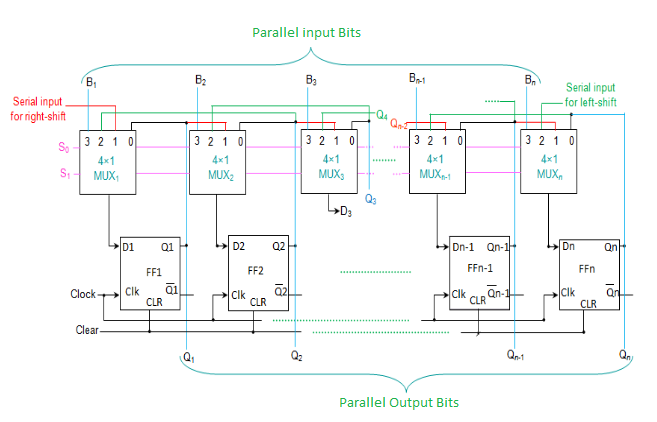
\includegraphics[width=0.8\textwidth]{imagens/universal shift register.png}
    \caption{Registrador de Deslocamento Universal (Fonte: Acervo Lima)}
    \label{fig:universal_sr}
\end{figure}

A palavra "UEFS", por sua vez, para ser representada em bits, foi utilizado a lógica presente na figura \ref{fig:uefs_em_bits}. Cada registrador terá em seu conjunto de flip-flops, na configuração da entrada paralela padrão, o bit representante da palavra "UEFS". Cada linha de bits da figura \ref{fig:uefs_em_bits} está representada como entrada do registrador. Por exemplo, o registrador da linha 1 (L1) possui, nas entradas de seus 16 flip-flops, a seguinte sequência de bits: 1010111011101110, respectivamente. 

\begin{figure}[!h]
    \centering
    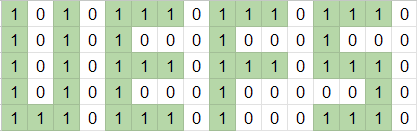
\includegraphics[width=0.5\textwidth]{imagens/palavra_em_bits.png}
    \caption{Representação em bits da palavra "UEFS"}
    \label{fig:uefs_em_bits}
\end{figure}

Cada flip-flop do tipo D recebe as seguintes entradas: ch0, ch1, para\_exibicao, dir\_esq, esq\_dir e CLK. Quando "para\_exibicao" for acionado (ch0 e ch1 em nível lógico baixo), os LEDs irão ser desligados e o registrador será setado com os valores iniciais pré-definidos. Quando "dir\_esq" for acionado (ch0 e ch1 em nível lógico alto e baixo, respectivamente), o flipflop atual vai receber a saída do flipflop anterior, ou seja, a exibição será feita da direita para a esquerda, pois será nessa orientação que os bits serão deslocados. Quando "esq\_dir" for acionado (ch0 e ch1 em nível lógico baixo e alto, respectivamente), o flipflop atual vai receber a saída do flipflop posterior, ou seja, a exibição será feita da esquerda para a direita, pois será nessa orientação que os bits serão deslocados. Por fim, quando ambas as entradas ch0 e ch1 forem nível lógico alto, o clock será inibido, ou seja, não haverá deslocamento e o painel será "pausado". O componente responsável por direcionar as entradas de seleção ch0 e ch1 para o flip-flop é o multiplexador. Por fim, os registradores enviam 7 saídas para a main, entituladas colunas, que são enviadas para a matriz de LEDs, que as selecionam através de um contador e um multiplexador.

Por sua vez, o módulo de matriz de LEDs é controlado por um contador e selecionador de linhas e colunas. O módulo recebe 2 sinais de entrada: ch0 e ch1, que são utilizados para habilitar ou desabilitar a matriz de LEDs. Há também um sinal de entrada CLK para sincronizar a operação do contador. Além disso, existem 35 sinais de entrada (C1L1, C1L2, ..., C7L5) que controlam os LEDs individuais e 12 sinais de saída (L1, L2, L3, L4, L5, C1, C2, C3, C4, C5, C6, C7) que são conectados aos pinos do componente físico.

O módulo utiliza um contador (Contador inst1) para selecionar a linha e a coluna correspondente que deve ser exibida na matriz de LEDs de maneira sicronizada. O contador gera três sinais de saída (en1, en2 e en3) que são usados para selecionar a linha e a coluna correspondente. A linha é selecionada com as portas lógicas AND que produzem um sinal alto (1) em cada linha correspondente selecionada, enquanto que as colunas são selecionadas por multiplexadores (MUXParaColuna) que conectam as saídas de cada coluna correspondente aos pinos de saída da matriz de LEDs.

O módulo também inclui uma função de habilitação/desabilitação, onde o sinal de saída "enable" é controlado pelos sinais de entrada ch0 e ch1. Se ambos forem zero, o "enable" é definido como zero, o que desabilita a matriz de LEDs. Caso contrário, o "enable" é definido como um sinal lógico alto (1), o que habilita a matriz de LEDs.

\begin{figure}
    \centering
    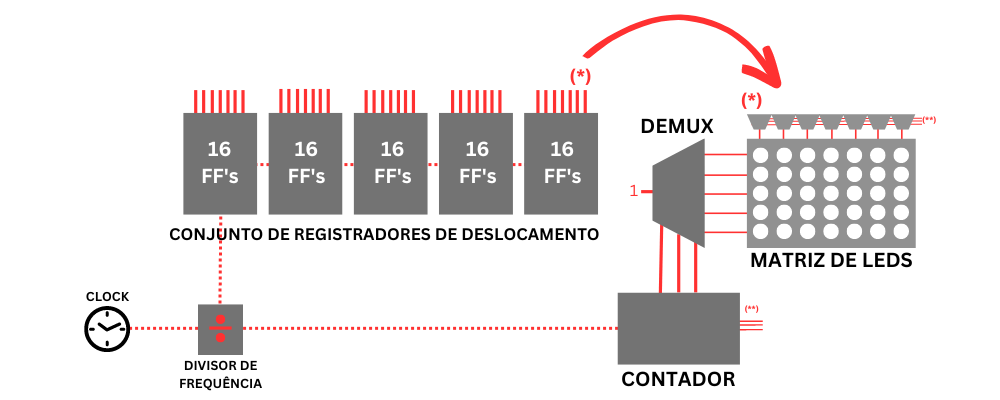
\includegraphics[width=0.9\textwidth]{imagens/design letreiro.png}
    \caption{Modelagem do circuito completo do painel eletrônico digital}
    \label{fig:modelagem}
\end{figure}

\section{Implementação física}

A implementação do código escrito em Verilog deve ser repassada para os circuitos integrados de lógica programável complexa (CPLD) para utilização do protótipo físico. 

Os CPLDs tem um funcionamento interno semelhante, mas mais complicados, aos integrados PAL e PLD. No CPLD existem vários sub-circuitos interconectados por uma matriz programável de interconexão global. Esses sub-circuitos recebem a nomenclatura de Logic Array Blocks (LABs) (Figura \ref{fig:diagramadeblocos}). Cada LAB contém blocos de I/O (entrada/saída), um circuito de expansão de termo produto e a quantidade de 4 a 16 macrocélulas. Cada macrocélula é estruturada com uma matriz AND conectada a uma matriz OR, para a implementação de soma de produtos, e flip-flops que, em alguns casos, são responsáveis pela realimentação de sinais na matriz AND \cite{CLPDarquitetura} O modelo utilizado foi o CPLD MAX II EPM240T100C5N.

Quando o código é ainda compilado no Quartus, uma série de informações acerca da implementação são geradas. No resumo do uso de recursos do Fitter, é possível ver todas essas informações. A partir do código apresentado neste relatório, temos as seguintes informações: 120/240 (50\%) elementos lógicos foram utilizados, todos no modo normal. Desses, no uso de elemento lógico por número de entradas LUT, 82 são de 4 entradas, 9 são de 3 entradas, 3 são de 2 entradas e 26 são de 1 entrada. Por fim, são utilizados 15 pinos, de 80 disponíveis (19\%).

\begin{figure}[!h]
  \centering
    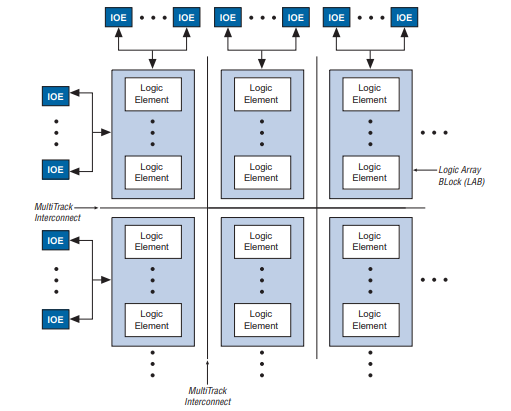
\includegraphics[width=0.45\textwidth]{imagens/diagrama.png}
  \caption{Diagrama de blocos do dispositivo MAX II}
  \label{fig:diagramadeblocos}
\end{figure}

\section{Teste e simulação}

Para realizar os testes físicos na placa, é recomendável realizar algumas simulações virtuais inicialmente e testar as saídas, na tentativa de perceber os problemas antes de estarem conectadas na placa. Caso a simulação esteja correta, o ideal é que a aplicação física tenha um resultado adequado. 

No momento de testes na placa, foi percebido uma anômalidade, onde os bits eram deslocados, mas não eram exibidos na matriz de maneira que desse para efetuar a leitura. Com uma análise, o problema foi visto na frequência que os bits eram exibidos. Em um divisor de frequência incial, os bits não eram exibidos adequadamente. Para verificar se o problema era realmente no divisor de frequência, uma saída foi forçada para o relé do kit de desenvolvimento LEDS CPLD, que foi conectada ao osciloscópio. Com isso, foi analisado que o clock do sistema não estava sendo dividido. Um erro foi diagnosticado no código e corrigido. Após isso, os testes foram validados e executados de maneira esperada, como demonstrada a seguir:

\begin{equation} \label{eqCLK2}
    x=\frac{50000000}{2^5}
\end{equation}

\begin{figure}[!h]
    \centering
    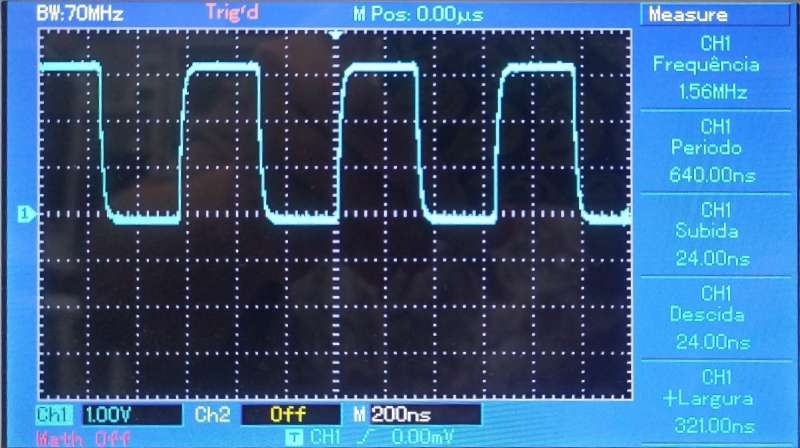
\includegraphics[width=0.6\textwidth]{imagens/osci01.jpg}
    \caption{Teste da divisão de frequência em 5 Flip-Flops feito no osciloscópio.}
    \label{fig:osci5}
\end{figure}

Dividindo o clock em 5 Flip-Flops, como demonstrado na equação \ref{eqCLK2}, para a sua utilização na matriz de LEDs, o resultado chega a 1562500Hz, ou 1,56MHz. A figura \ref{fig:osci5} demonstra o teste feito utilizando o osciloscópio. Para a realização do teste, foram utilizadas as saídas do relé do kit de desenvolvimento (LEDS CPLD). Essas saídas foram conectadas ao osciloscópio para demonstração da divisão do clock.

\begin{equation} \label{eqCLK3}
    x=\frac{50000000}{2^2^3}
\end{equation}

\begin{figure}
    \centering
    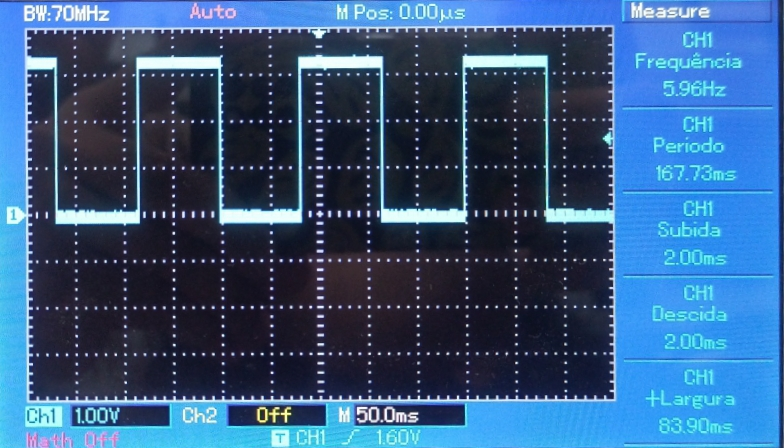
\includegraphics[width=0.6\textwidth]{imagens/osci02.jpg}
    \caption{Teste da divisão de frequência em 23 Flip-Flops feito no osciloscópio.}
    \label{fig:osci23}
\end{figure}

Já o clock que foi utilizado para o registrador de deslocamento, precisou ser utilizar 23 Flip-Flops no divisor de frequência, como demonstrado na equação \ref{eqCLK3}, com o resultado chegando a aproximadamente 5,96Hz. O resultado precisa ser menor que o clock de exibição da matriz pois o deslocamento precisa ser percptível referente a sua exibição. A figura 6 demonstra o teste feito utilizando o osciloscópio.




\chapter{RESULTADOS}
O protótipo passou por alguns problemas de implementação que foram corrigidos depois de algumas discussões e sessões. Entretanto, por fim, após realizar as simulações e todos os testes possíveis depois da implementação, foi considerado o preenchimento de todos os requisítos solicitados. O protótipo cumpre com maestria a conversão do código 2 de 5 em decimal, manipula o display de sete segmentos e a matriz de LEDs e lida com o erro nas variadas situações possíveis.

Por outro lado, a equipe aprendeu a manipular os códigos de descrição de hardware no mais baixo nível, relacionando-o com as variadas funções lógicas de saídas. Ademais, desenvolveu habilidade de interpretação, manipulação e conversão de alguns códigos númericos existentes e de reconhecimento de padrões e relações entre portas lógicas, desenvolvendo decodificadores e multiplexadores.

De forma adicional, mas fora do que foi solicitado, o projeto poderia passar por atualizações para importação de um módulo que lidasse com a leitura real do código de barras, além da inserção manual do código. Ainda dentro do tema proposto, ao invés de simplemente converter, poderia armazenar os dados lidos e manusear o possível gerenciamento desses dados. 



\postextual
\endgroup

% ----------------------------------------------------------
% Referências bibliográficas
% ----------------------------------------------------------
\bibliography{bibliografia}

\end{document}
